% Appendix A
\section{ZigBee Additions}%XBee join and send time experiments} % Main appendix title
\label{AppendixA} 

\subsection{ZigBee Stack}
\begin{figure}[htbp]
\centering
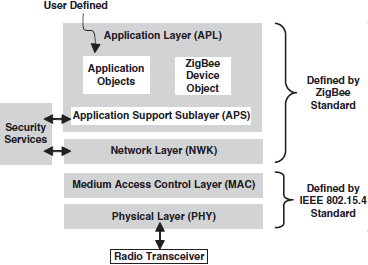
\includegraphics[width=0.58\textwidth]{stack}
\caption{ZigBee Protocol Layers ( $\circlearrowleft$ \ref{lab1} )}
\label{fig:stack}
\end{figure} 

%--------------------------------------------------

\subsection{Logical Device Types}
\begin{figure}[htbp]
\centering
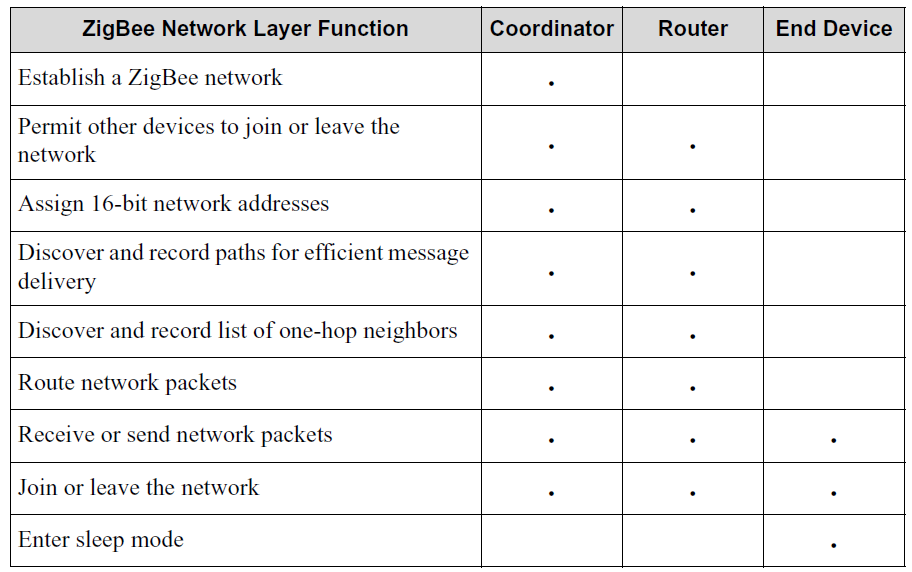
\includegraphics[width=0.78\textwidth]{roles}
\caption{Comparison of ZigBee Devices at the Network Layer ( $\circlearrowleft$ \ref{lab2} )}
\label{fig:roles}
\end{figure} 

%---------------------------------------------

\newpage
\pagebreak
\clearpage
\subsection{ZigBee Sleep Mode}
\label{zigbeesleep}
\subsubsection{Waspmote V1.1}
As mentioned in section \ref{lab5}, the current Waspmote program has the possibility to enable ZigBee / XBee sleep via the following definitions, accessible in 'PowerUtils.h' and the Libelium IDE, but will not use ZigBee sleep in default configurations.
\usestyle{vs} 
\includecode{sleep.cpp}

\noindent
This decision is based on the next conclusions related to the \verb+XBeeSleepMode+:
\begin{enumerate}
\item \textbf{Waspmote V1.1 has no support for wakening from ZigBee cyclic sleep}: When the Waspmote and the XBee are in sleep, the XBee should be able to wake the Waspmote when it detects his parent has a message pending for it. This is possible via a new interrupt routine added to Waspmote PRO. To do this on the first version one must solder pin 13 of the XBee to the MUX\_RX pin of the Waspmote. This way interruptions caused by the XBee module can be captured, but all other interruption options will be masked by pin 13's output and will thus be lost.
\item Enabling ZigBee sleep removes the association delay (see section \ref{second} ) but \textbf{requires 5 - 20 extra seconds to retrieve messages which are pending in the parent's buffer}. This has a very negative impact on battery life since all this time the XBee is turned on and receiving.
\item There is no guarantee that pending messages will be found when the Waspmote checks for them or in which order they will be received, so \textbf{network stability can no longer be guaranteed}. For example, when a privileged web interface user changes a sensor's measuring interval at minute 0 and another user re-changes the interval at minute 1, it is possible the request of the first user will be received after the request of the second user, so the node will not have the correct settings. This could be solved by adding timestamps to the requests or comparing the nodes responses with the web interfaces values. \item \textbf{Adding timestamps can help, however it is still possible that requests will go lost}. This happens from sleeping times of 15 seconds and more. This means that firstly the node will be much more active than sleeping. Secondly, the goal of using ZigBee sleep was to speed up the network response time and since packets can go lost due to enabling ZigBee sleep the network's response is worse than without using ZigBee sleep.
\end{enumerate}
\vspace{0.5cm}
\noindent
By checking for received messages immediately after sending sensor data, we can:
\begin{enumerate}
\item Guarantee network stability and disable ZigBee sleep
\item Save battery life by:
\begin{itemize}
\item Shorter duty cycles because we know when a message can be received
\item No XBee sleep current
\end{itemize} 
\end{enumerate}

%----------------------------
\subsubsection{Waspmote PRO} %to appendix
A sleeping Waspmote PRO can be interrupted when its sleeping XBee notices its parent has RF data available. The next paragraphs will briefly discuss the ZigBee protocol and settings.. 
\paragraph{ZigBee Sleep: Managing End Devices}
ZigBee end devices are intended to be battery powered and are capable of sleeping for extended periods of time. Because of this, routers and coordinators use packet buffers and transmission timeouts to ensure reliable data delivery to end devices.\\
When an end device joins the network, a parent-child relationship is formed with a router or the coordinator. From then on, if the end device is awake, it will send poll request messages (by default every 100 ms) to its parent to determine if the parent has any data buffered for it, independent of the sleep mode. Routers buffer this data only up to 28 - 30 seconds, so if we want to ensure reliable communication, this is the maximum sleep time. The child poll timeout can however be set up to a couple of months, so an end device can sleep longer than 30 seconds and still be considered to be in the network. This includes the node is associated within a few milliseconds, compared to the 2.5 seconds mentioned in section \ref{startup}. End devices can choose between two sleep modes, discussed in the next sections. 
\paragraph{Pin sleep}
In this mode an external microcontroller controls when the XBee should sleep and when it should wake by controlling pin 13. The module will not respond to serial or RF data when it is sleeping.\\\\
\textbf{+} lowest power consumption\\
\textbf{+} external controller can take samples without powering up the radio\\
\textbf{-} ZigBee protocol has less control\\
\textbf{-} external controller's timer is not accurate enough to synchronize the network\\
\textbf{-} Need fully awake parent\\
\paragraph{Cycle sleep}
Allows the XBee to determine when to wake up. The module can sleep for a specified time and wake for a short time to poll its parent for buffered data. If the parent has date the device will remain awake for a time, otherwise it will re-enter sleep mode immediately. 
\begin{itemize}
\item + suitable for DigiMesh, where the sleep clocks is accurate enough to get all nodes awake at the same time
\item + with DigiMesh, fully awake routers are not required, so they can be battery powered
\item - more power consumption due to accurate clock
\item - external controller must also wake when the XBee wakes to treat potentially received messages, even if there is no need to sample data
\end{itemize}

\paragraph{XBee sleep parameters}
\textbf{Router/Coordinator Configuration:} 
\begin{itemize}
\item RF Packet Buffering Timeout: 
\begin{itemize}
\item Sleep Period (SP) parameter. Max 30 seconds.
\item For cyclic sleep devices: SP should be set the same on routers and coordinators as it is on cyclic sleep end devices
\item For pin sleep devices: SP should be set equal to the time the end device can sleep, up to 30 seconds. If an end device sleeps longer than 30 seconds, parent and possibly non-parent devices must know when the device is awake. Therefore and devices that sleep longer than 30 seconds should transmit some kind of data (API frame) to alert the other devices that they can send data to the end device.
\end{itemize}
\item Child Poll Timeout: Sleep Number (SN) parameter: The number of Sleep Periods (SP) used to calculated end device poll timeout.
\end{itemize}

\vspace{0.5cm}
%--------------------------------------------------------------------
\subsection{Sleeping Mesh}
What is \textit{really} low power about ZigBee? The answer is already deducible from the previous sections, namely End Devices! A sleeping mesh tries to establish a multi-hop mesh network and low power routing functionality in one system, also using battery-powered routers. The system has two big requirements however:
\begin{itemize}
\item very low bandwidth, high latency
\item static network
\end{itemize}
For example, delivery of one data packet from every node every 12-24 hours, with a wake period of about 15 seconds. In a sleeping mesh all nodes wake up simultaneously and periodically to exchange and or route data. Afterwards, all nodes except the coordinator go back to sleep, a state which they are in 99\% of the time. In such a set-up battery lifes of 10 years and more are easy to reach.
\vfill
\pagebreak
%--------------------------------------------------------------------
\subsection{Range Test}
This procedure describes the easiest way to perform a range test using X-CTU. The test requires one coordinator node and one router node configured in AT mode.\\

\begin{enumerate}
    \item Set the target module address in both radios, as indicated in figure \ref{range1}.
    %\item To discuss digital systems of this scale and level of complexity
    %we need a number of descriptive tools.
    %\item For example:                                                 
    \begin{itemize} %label=\alph*)]
        \item item Module A will have the address of B in its destination field.\par
        \item Module B will have the address of A in its destination field. \par
        \begin{minipage}{\linewidth}
            \centering
            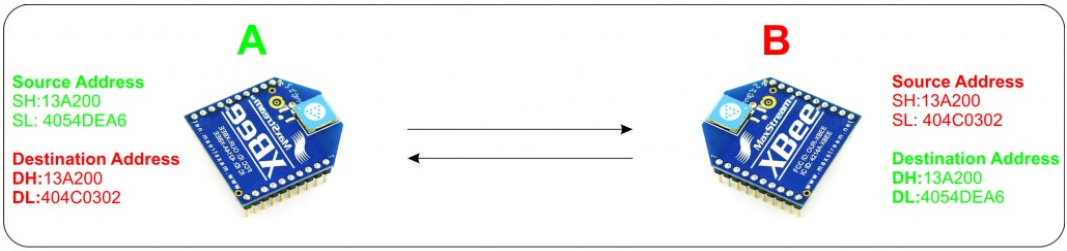
\includegraphics[width=12cm]{range1}
            \captionof{figure}{XBee Address Exchange}
            \label{range1}
        \end{minipage}
        %\item Timing diagrams highlight the detailed time sequence of
        %transfer between registers.\par
        %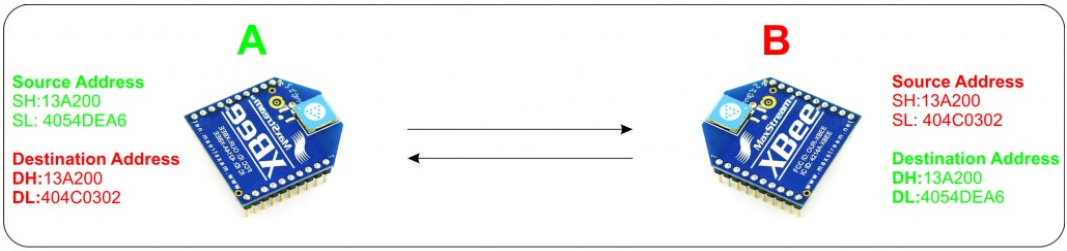
\includegraphics[width=10cm]{range1}
    \end{itemize}
    \item Make sure the modules have the same PAN ID and CHANNEL settings and write the values to the XBees.
    \item To do the range test, a data packet will be send and the module expects the same packet to be received:
	\begin{itemize}
		\item Connect the sending module to your laptop, e.g. module A. \par
		\item Module B must not be connected to any device but its Rx and Tx pin (XBee pin 2 and 3) must be connected to each other in order to create the loopback connection. To do this you can use a small breadboard. See figures \ref{range2} and \ref{range3}. \par
        \begin{minipage}{\linewidth}
            \centering
            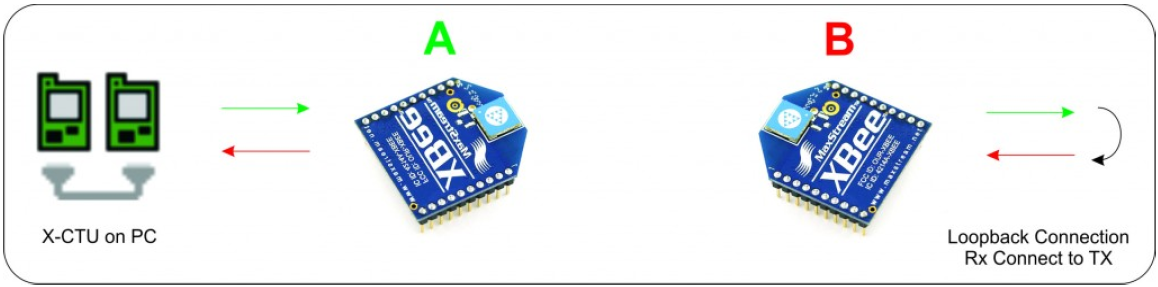
\includegraphics[width=12cm]{range2}
            \captionof{figure}{XBee Loopback Test}
            \label{range2}
            \vspace{1cm}
            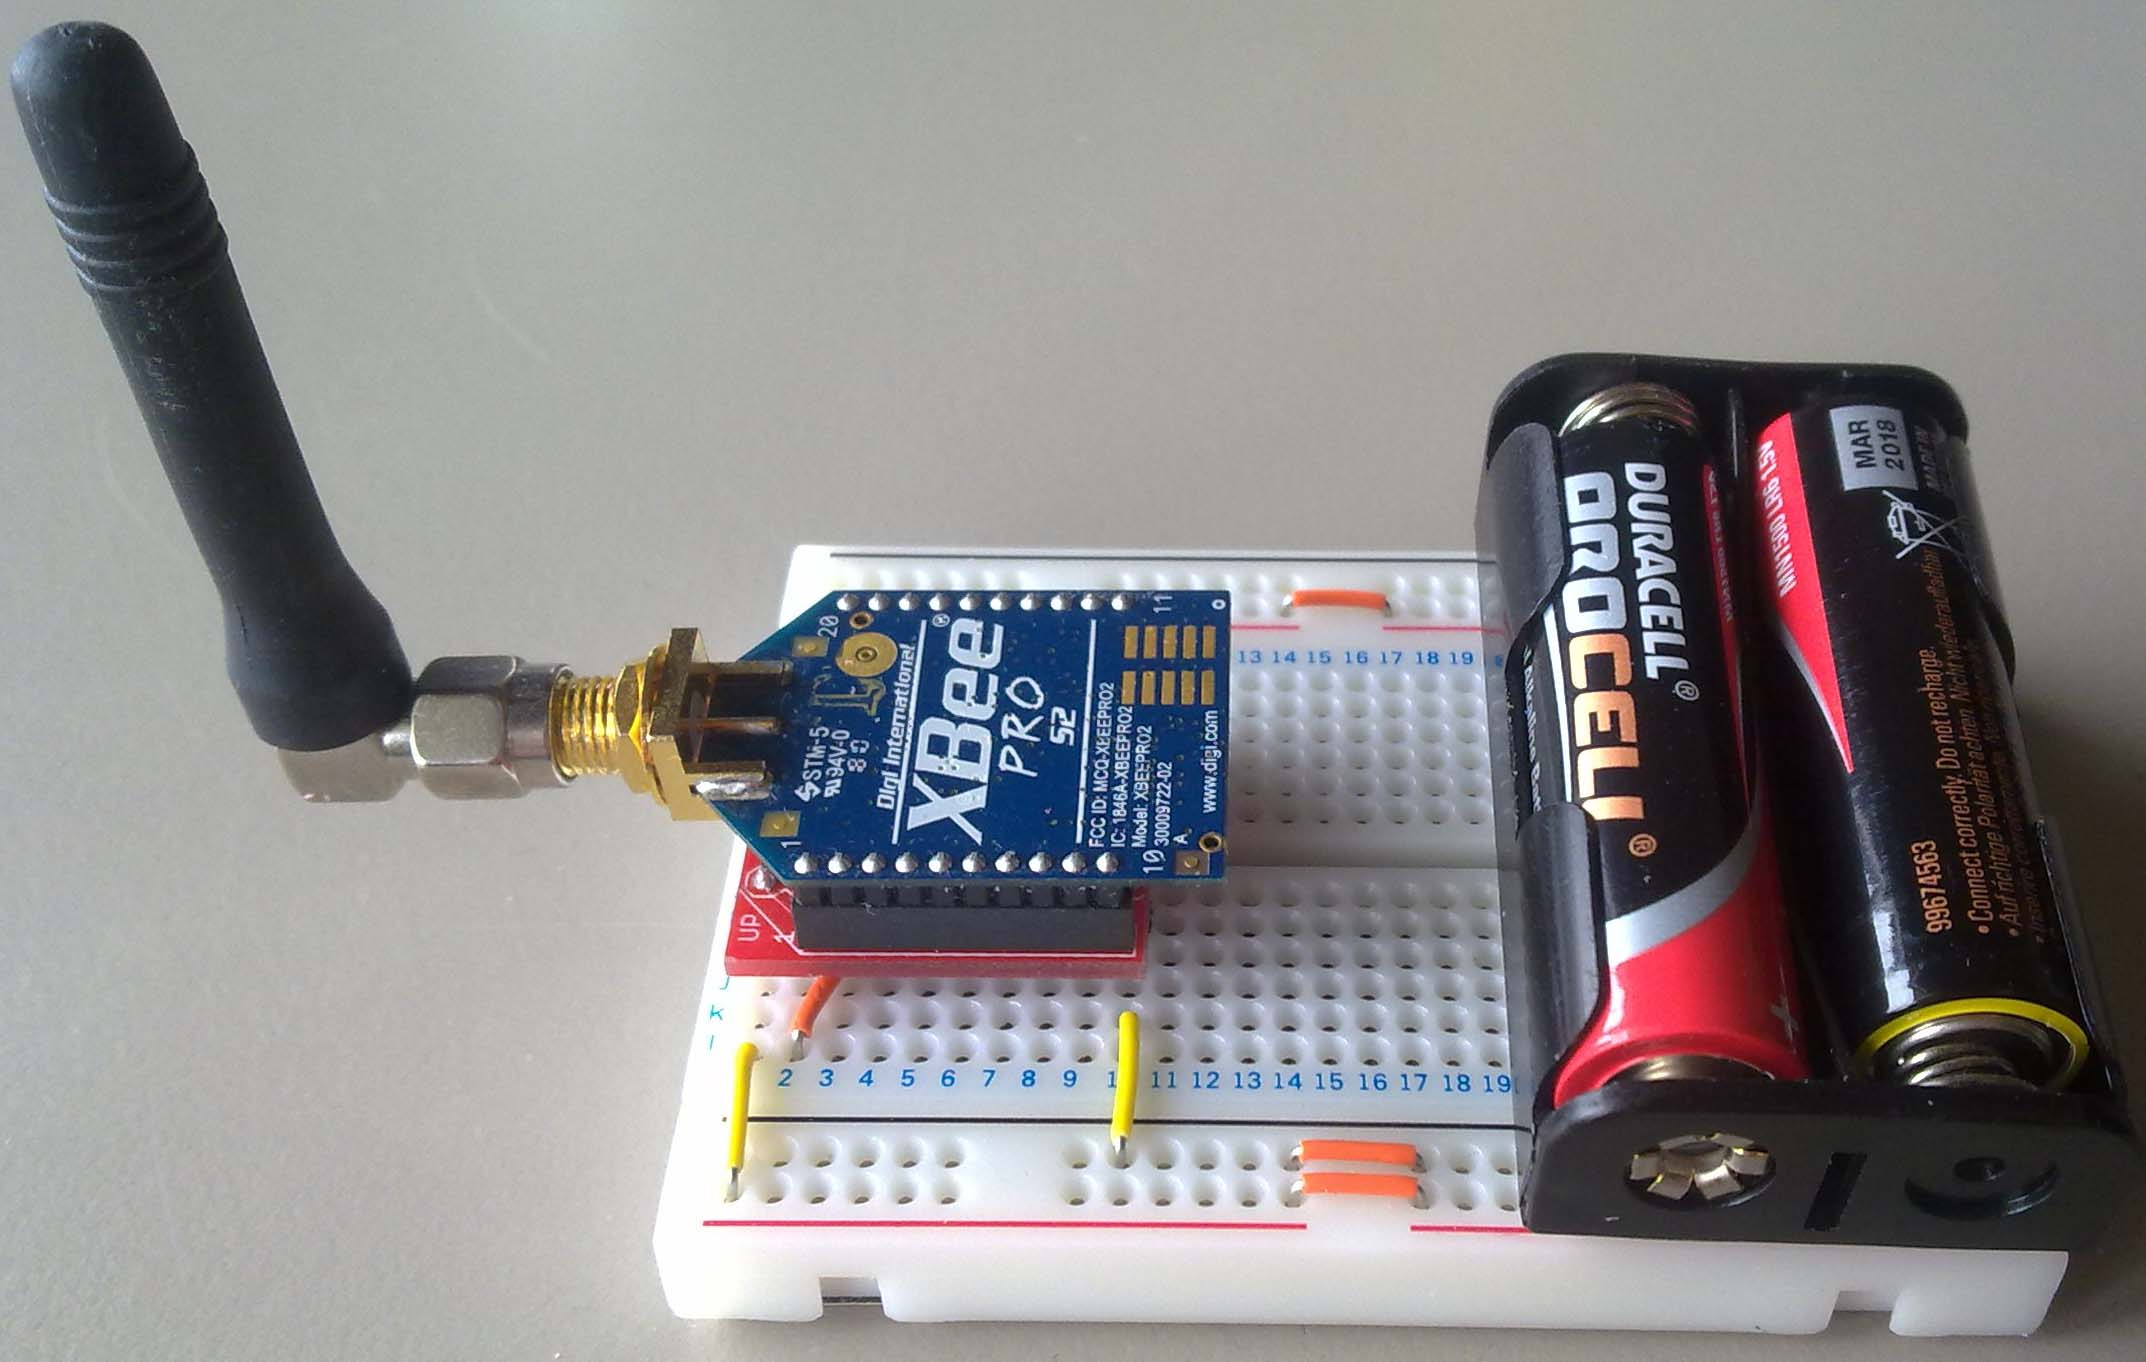
\includegraphics[width=12cm]{range3}
            \captionof{figure}{Module B Loopback Connection}
            \label{range3}
        \end{minipage}		
     \end{itemize}
     \vfill
     \pagebreak
     \item Go to the \textit{Range Test} tab in X-CTU, \textbf{select the checkbox under RSSI} and click \textit{Start} to run the test. Leave module B at a fixed position and walk around with your laptop to immediately see the RSSI value. Your screen should look as indicated in figure \ref{range4}. \par
             \begin{minipage}{\linewidth}
            \centering
            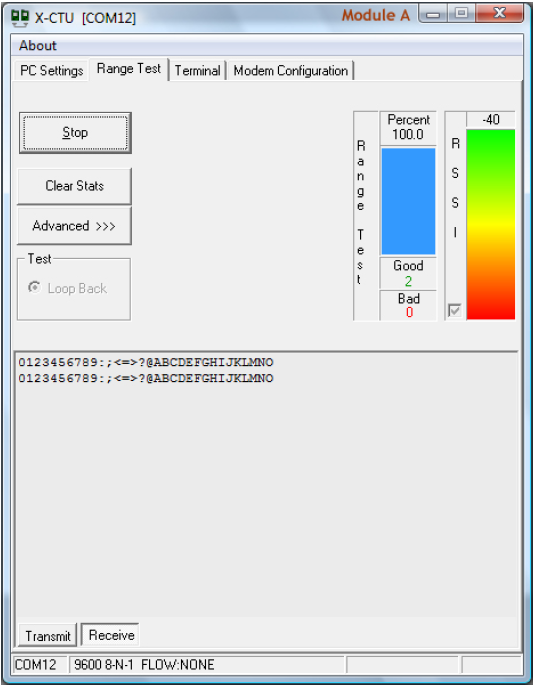
\includegraphics[width=10cm]{range4}
            \captionof{figure}{X-CTU Range Test}
            \label{range4}
        \end{minipage}
\end{enumerate}

\vfill
\pagebreak
\subsection{Self-made mobile XBee ZigBee node}
\label{mob}
\begin{figure}[htbp]
\centering
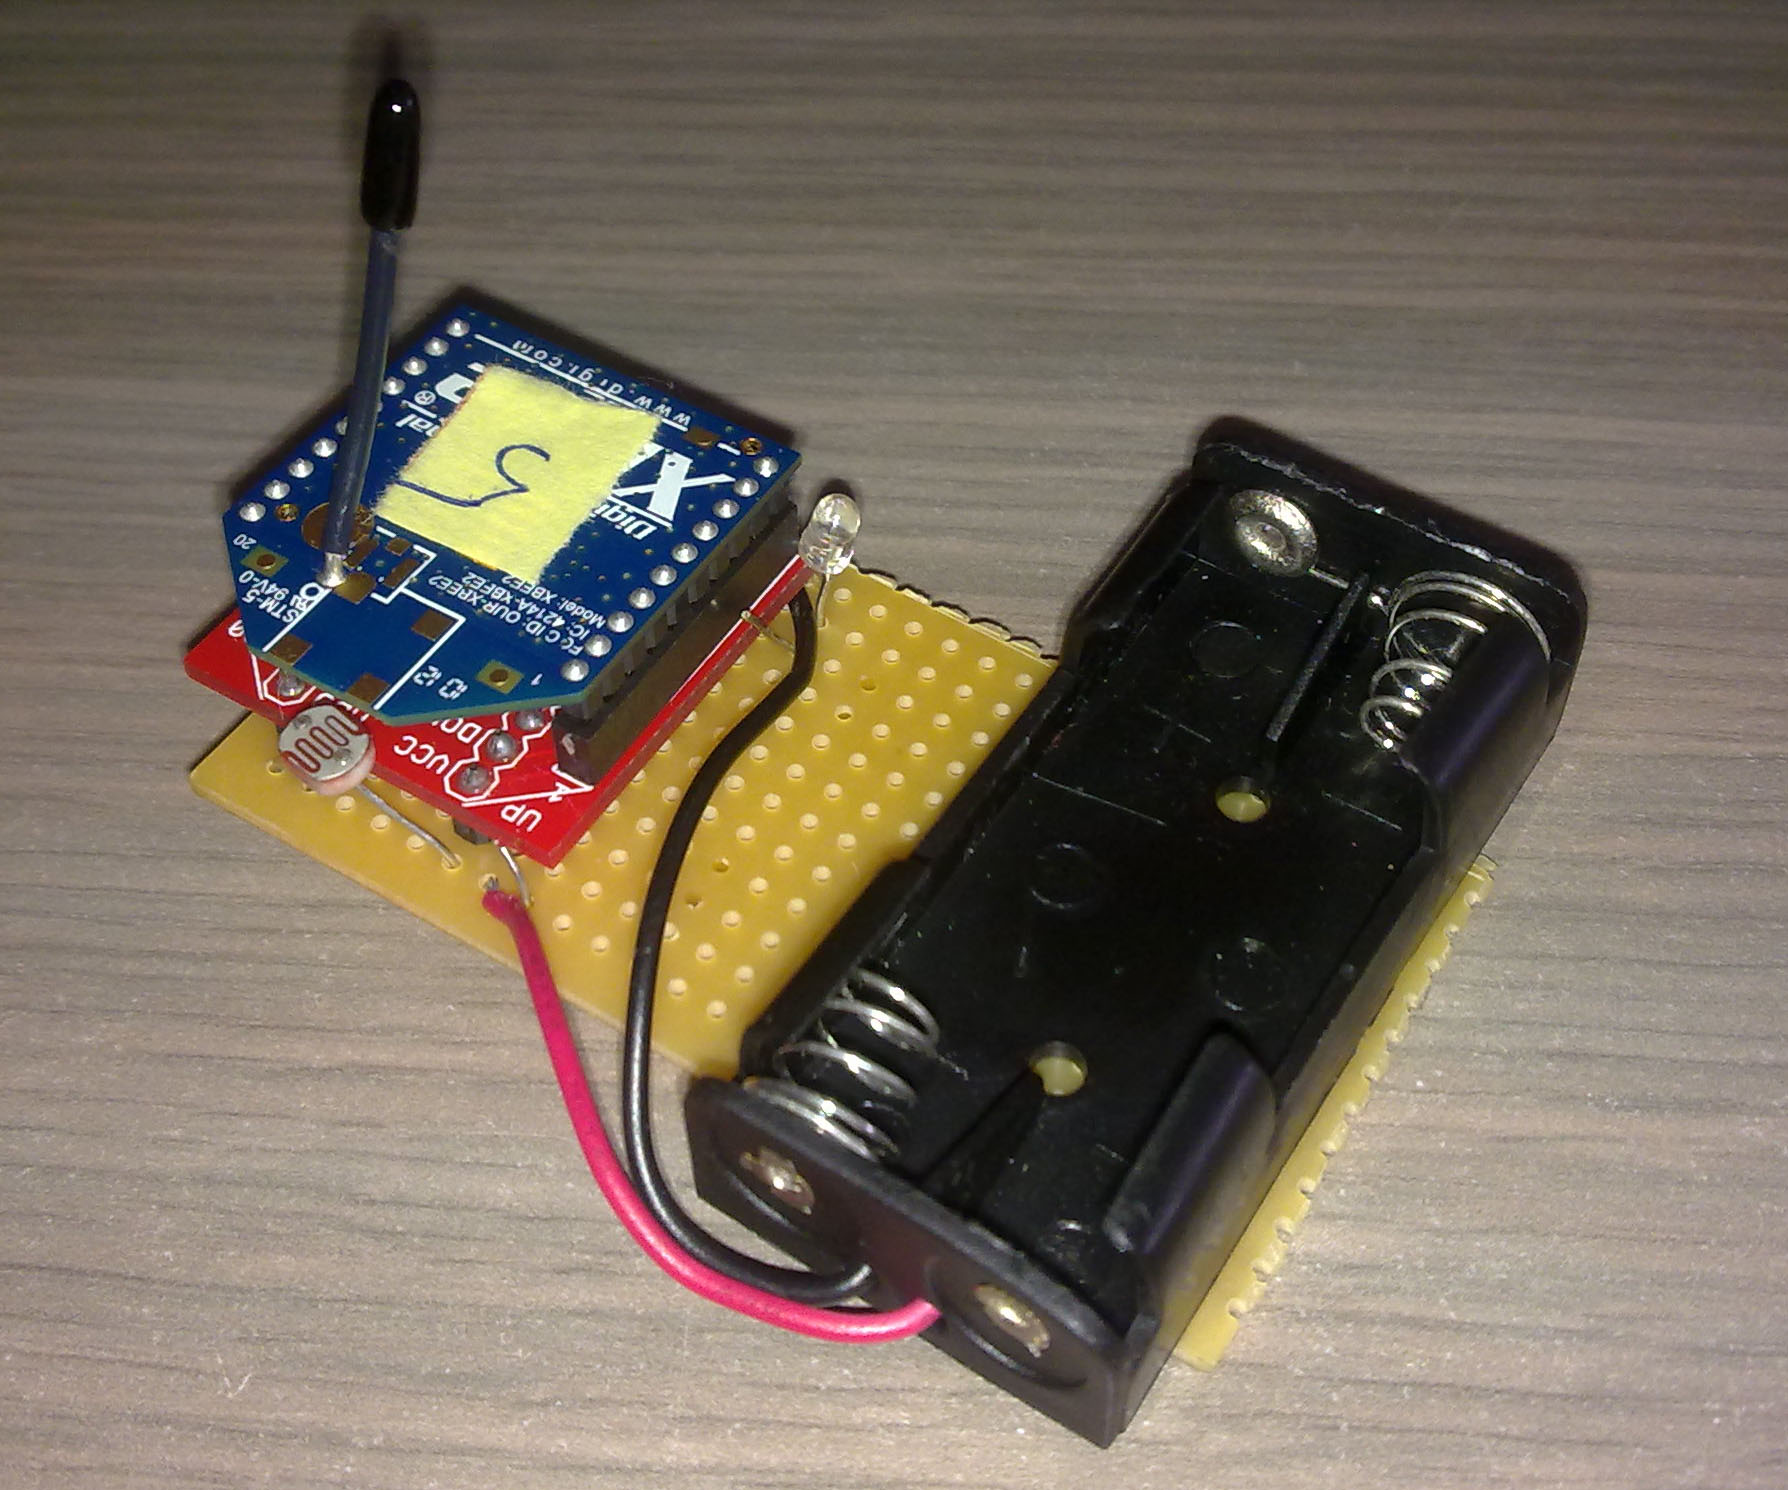
\includegraphics[width=0.78\textwidth]{mob}
\caption{A simple mobile node}
\end{figure} 